\documentclass[UTF8,a4paper]{ctexart}

% --- Common packages ---
\usepackage{amsmath,amssymb,amsfonts,mathtools}
\usepackage{amsthm}
\usepackage{bm}
\usepackage{graphicx}
\usepackage{siunitx}
\usepackage{booktabs}
\usepackage[margin=2cm]{geometry}
\usepackage{float}
\usepackage{caption}
\usepackage{hyperref}
\usepackage{cleveref}
\usepackage{listings}
\usepackage{tikz}
\usepackage{physics}
\usepackage{fancyhdr}
\pagestyle{plain}
\geometry{a4paper, left=2.5cm, right=2.5cm, top=2.5cm, bottom=2.5cm}
% --- Shortcuts / common macros ---
\providecommand{\dd}{\mathop{}\!\mathrm{d}}
\renewcommand{\vec}[1]{\boldsymbol{#1}}
\newcommand{\rme}{\mathrm{e}}
\newcommand{\rmi}{\mathrm{i}}
\newcommand{\rmj}{\mathrm{j}}

% --- Theorem environments ---
\newtheorem{theorem}{定理}[section]
\newtheorem{lemma}[theorem]{引理}
\newtheorem{proposition}[theorem]{命题}
\newtheorem{corollary}[theorem]{推论}
	\theoremstyle{definition}
\newtheorem{definition}{定义}[section]
	\theoremstyle{remark}
\newtheorem{remark}{注记}[section]

% --- title ---
\newcommand{\hwtitle}[2]{%
	\begin{center}
		{\huge\bfseries #1\par}
		\vspace{0.50em}
		{#2\par}
	\end{center}
	\vspace{0.6em}
}

\hypersetup{colorlinks=true,linkcolor=blue,citecolor=blue,urlcolor=blue}

% 正文部分
\begin{document}

% Edit the arguments below: {作业标题}{作者信息}
\hwtitle{于比特与原子间穿行}{姓名：何铭源 \quad 学号：3240104481 \quad 课程：工程导论}
\section{从知识的骨架到感性的血肉}
工程学是一门运用科学与数学，旨在解决现实问题的系统性学科。
这一定义如同一幅精确的蓝图，构筑了我对工程的初步认知。然而，知识的骨架终需感性的血肉来填充。
直至我亲身穿行于云栖大会的数字光影与上海工博会的钢铁森林之间，这幅蓝图才真正被赋予了生命、色彩与灵魂。
那是一场从云端到大地的壮丽巡礼，一场在比特的虚空中沉思、在原子的实体上触摸的探索。
我所追寻的，不仅是两个展会的见闻，更是对工程范畴的重新丈量，以及对工程未来命运的深切叩问。
\section{云栖大会}
我的旅程始于云栖大会，那是一个几乎由纯粹信息构筑的场域。
空气中流淌的并非尘埃，而是涌动的数据流与无形的计算力。
在这里，工程的传统边界被悄然溶解，其伟力不再仅仅体现于可触可感的物理建构，更在于编织无形的智慧服务与构建庞大的数字生态。
这场变革最鲜明的体现，便是人工智能如水银泻地般融入千行百业的肌理。它不再是象牙塔中的理论幻梦，而是化作了解决具体困境的强大工程实践。

在菜鸟网络的展区，我见证了其全球贸易关务助手如何将繁复化为简约。
\begin{figure}[H]
	\centering
	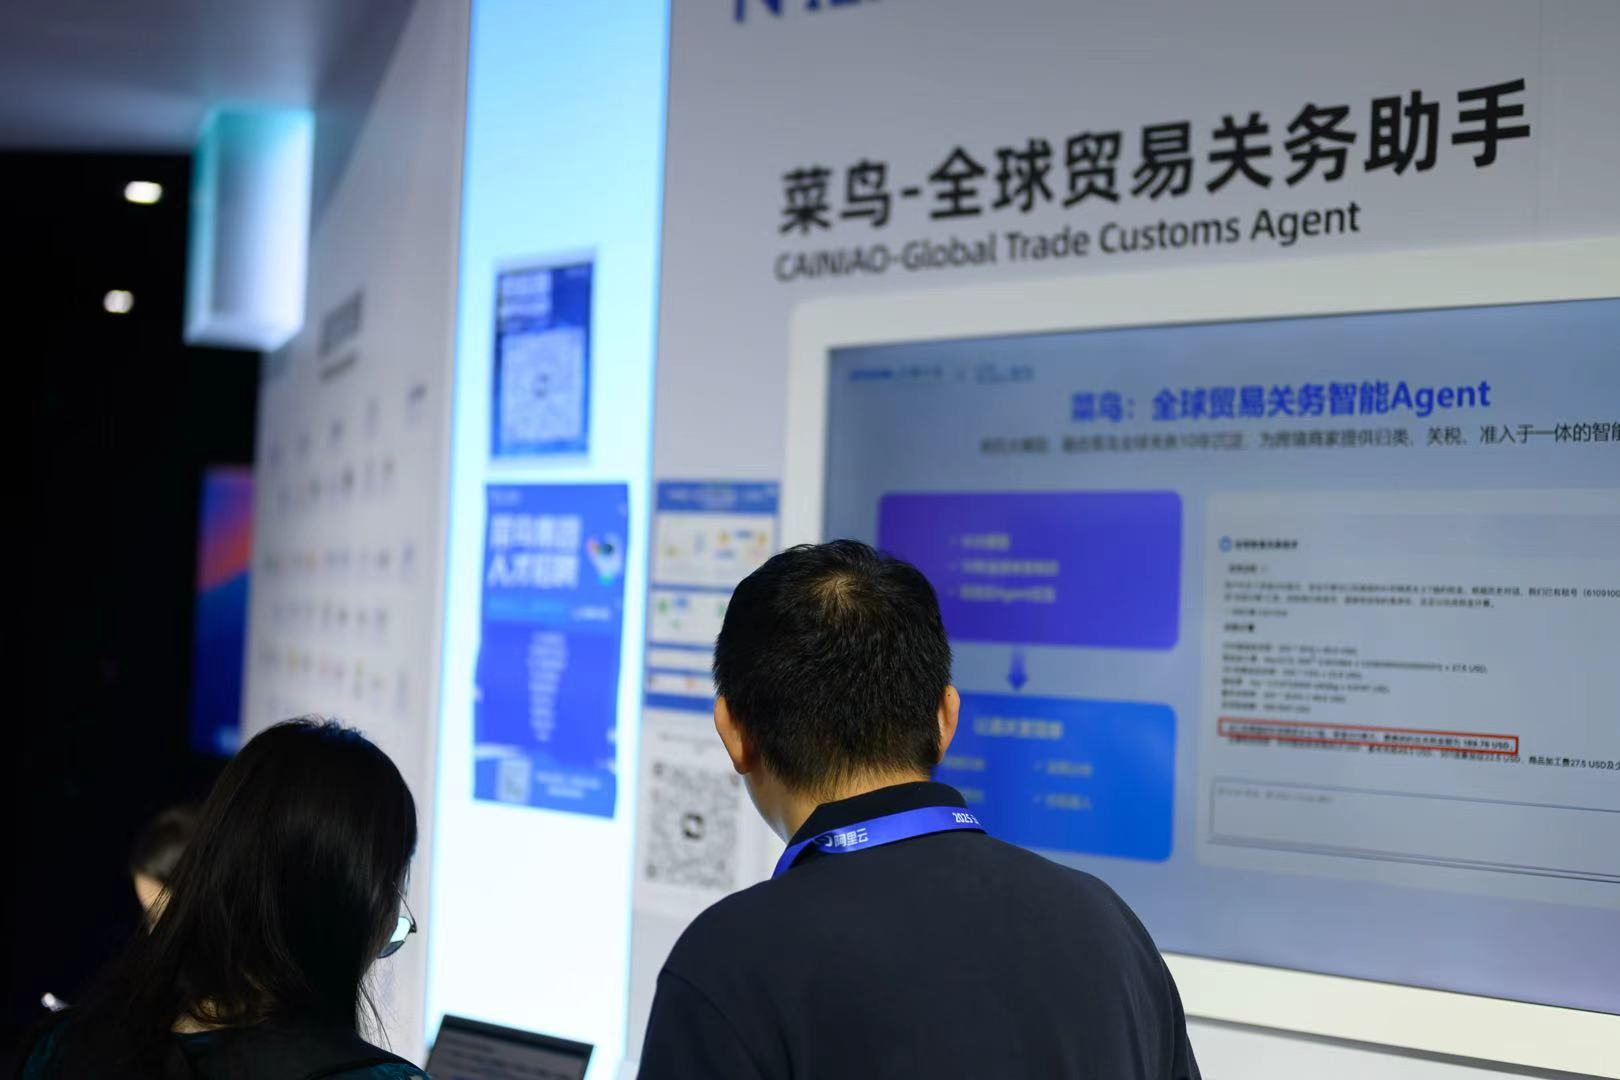
\includegraphics[width=.7\textwidth]{./fig/菜鸟.jpg}
	\caption{菜鸟与AI的结合}
\end{figure}
过去，一份跨国贸易单证的流转，意味着冗长的人工审核与潜在的错误风险；
而今，人工智能以其敏锐的视觉与深刻的语言理解力，瞬息之间便能完成单证解析、海关编码匹配乃至风险预警。
这背后，是一项恢弘而精密的智能工程。
工程师们在此扮演的角色，早已超越了传统程序员的范畴。他们是数据科学家、算法专家与系统架构师的集合体，致力于创造一种能够自我学习、持续进化的智慧服务。
这股力量同样赋能于直播、商务等无数场景，它们共同宣告了一个事实：工程的疆域，已从有形的物质世界，浩浩荡荡地延伸至无形的服务、知识与决策领域。

\begin{figure}[H]
\centering
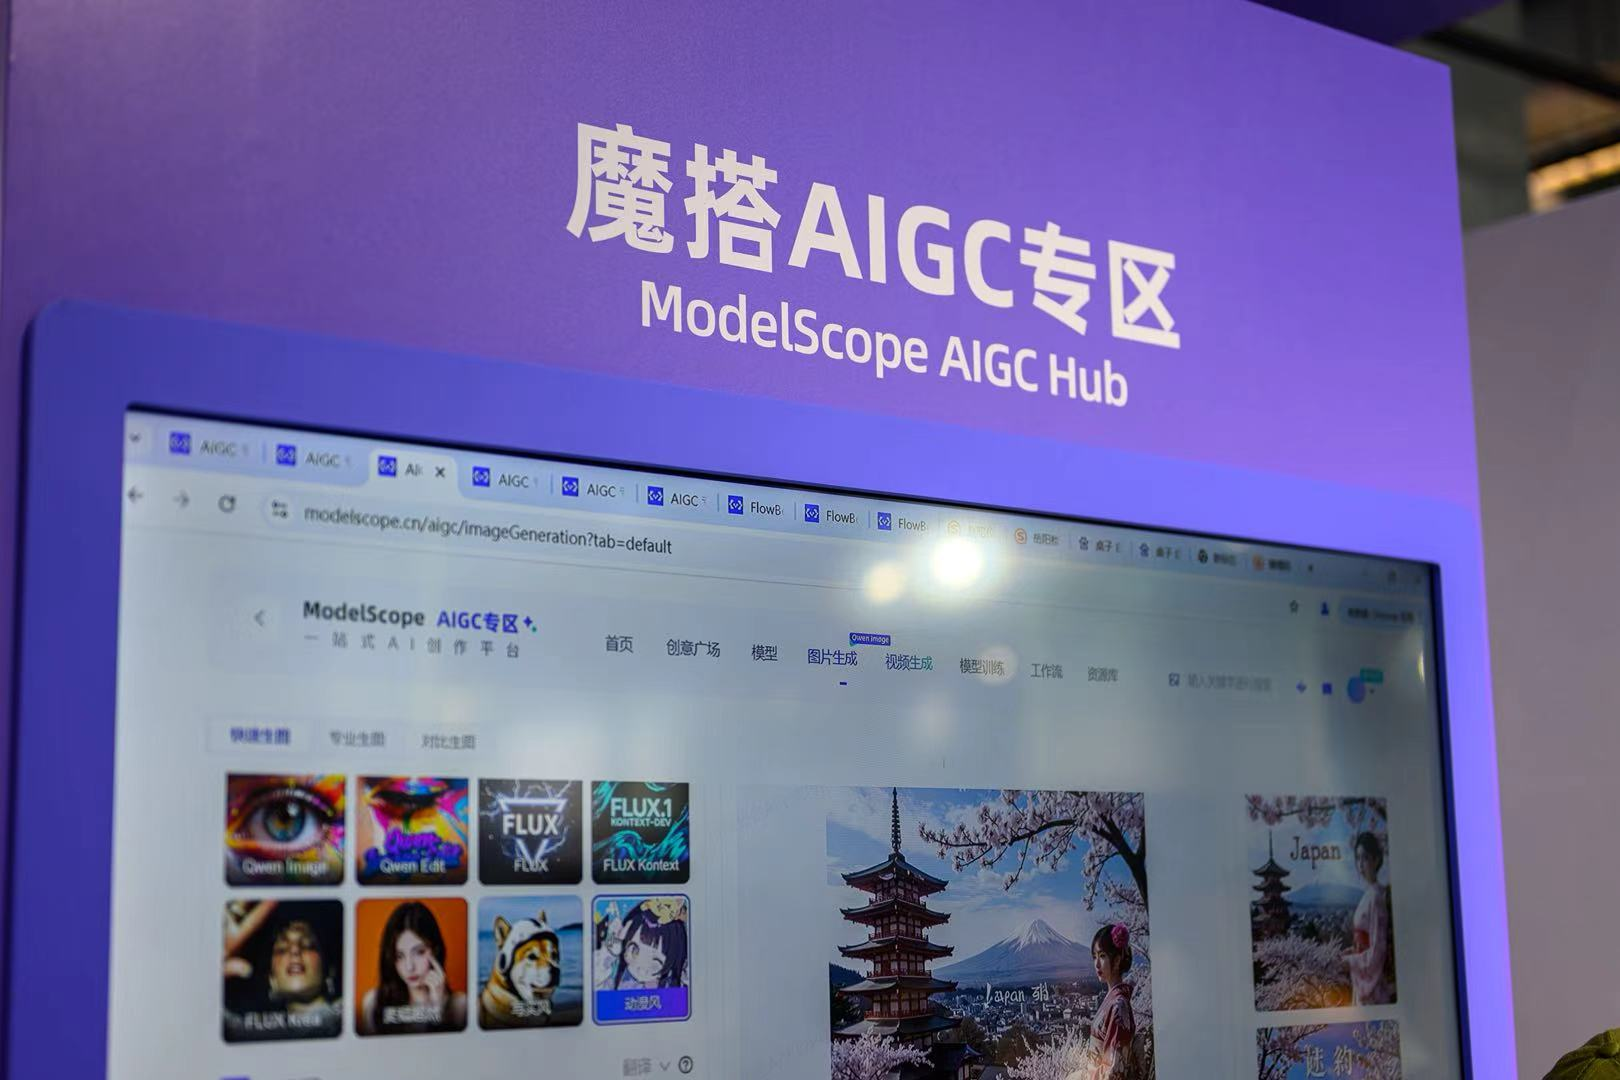
\includegraphics[width=.4\textwidth]{./fig/aigc.jpg}\quad
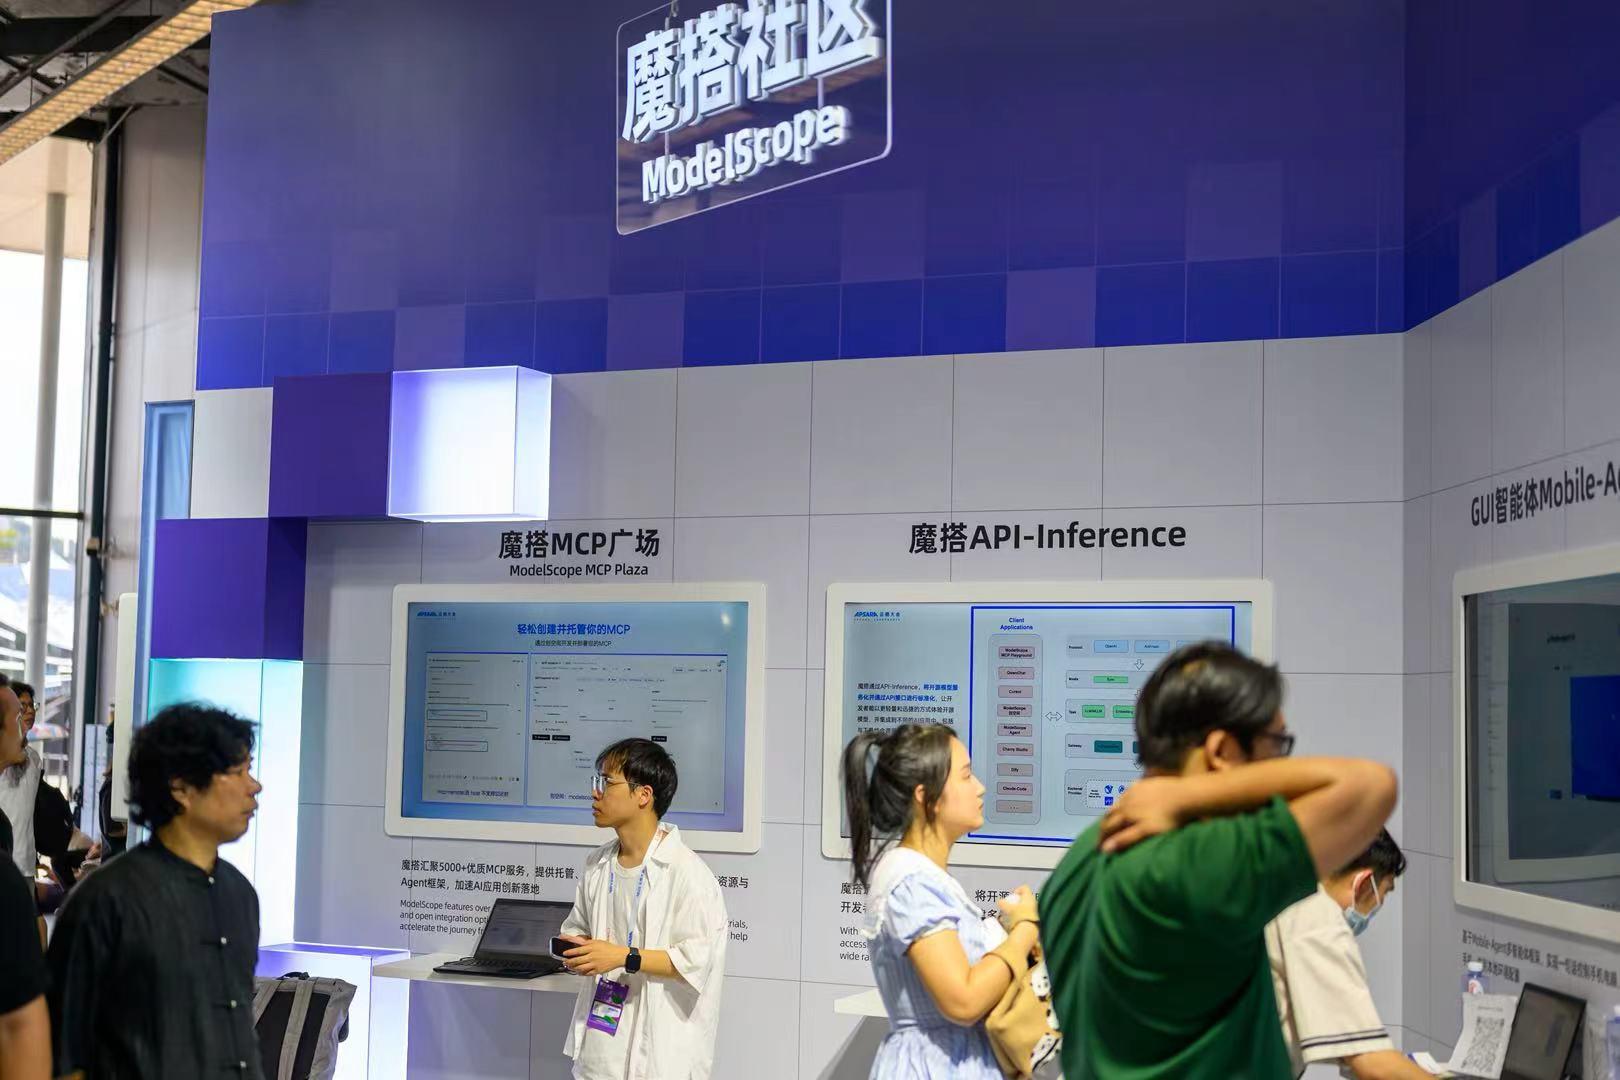
\includegraphics[width=.4\textwidth]{./fig/魔搭.jpg}
\caption{AI与各种场景结合，可以实现各种内容}
\end{figure}
\begin{figure}[H]
\centering
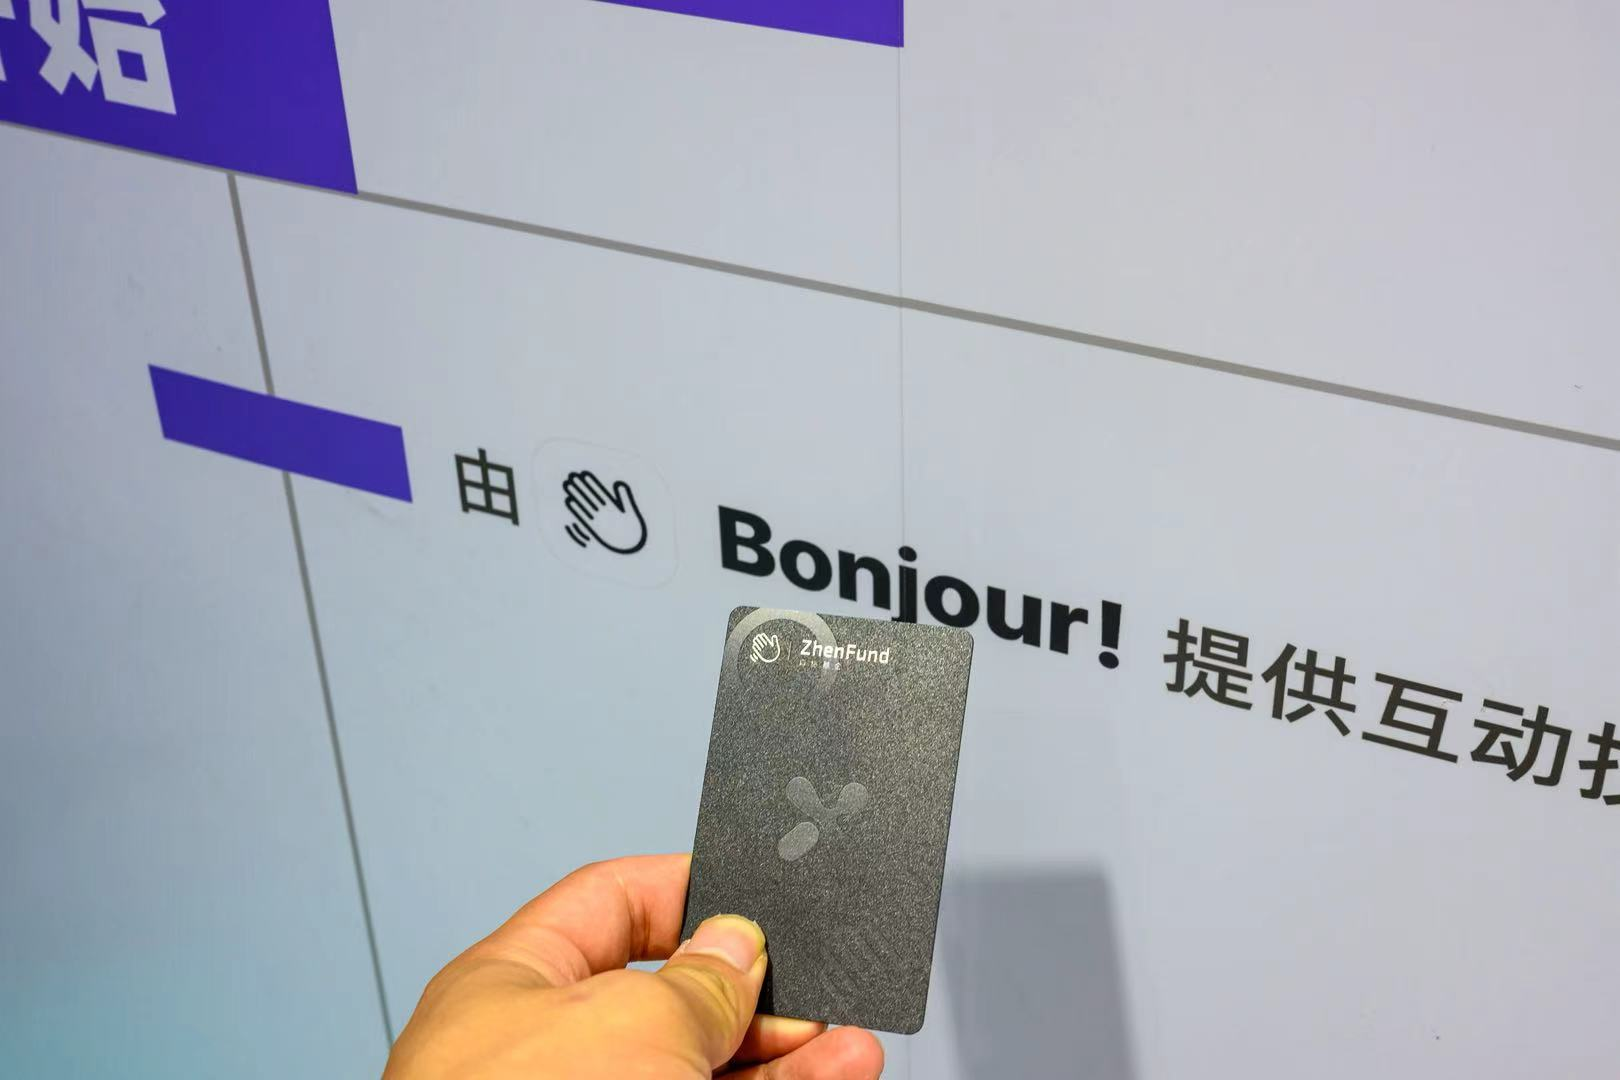
\includegraphics[width=.7\textwidth]{./fig/卡牌.jpg}\quad
\caption{个人名片与AI的结合，本人之前上创业实践课拿到过同款产品}
\end{figure}

若说这些应用是人工智能之树结出的累累硕果，那么阿里云发布的通义千问大模型，则让我得以窥见其深植于技术土壤中的庞大根系。
大语言模型本身，便是一座矗立于数字时代的工程学丰碑。
它的诞生，需要吞噬海洋般浩瀚的高质量数据，需要唤醒由成千上万枚高性能芯片构成的计算集群，并通过极度复杂的分布式系统协同运转。
模型的每一次迭代，都是算法、算力与工程实现等多个维度合力推动的交响。
我由此领悟，当代前沿工程，尤其是人工智能工程，是一种智力密度极高的系统性创造，其复杂与壮阔，丝毫不亚于构筑一座现实世界中的超级工程。

在对未来工程形态的探寻中，阿里云Qoder展台所揭示的，是一种名为vibe coding的全新编程范式，它几乎重塑了我对人机交互的想象。
\begin{figure}[H]
\centering
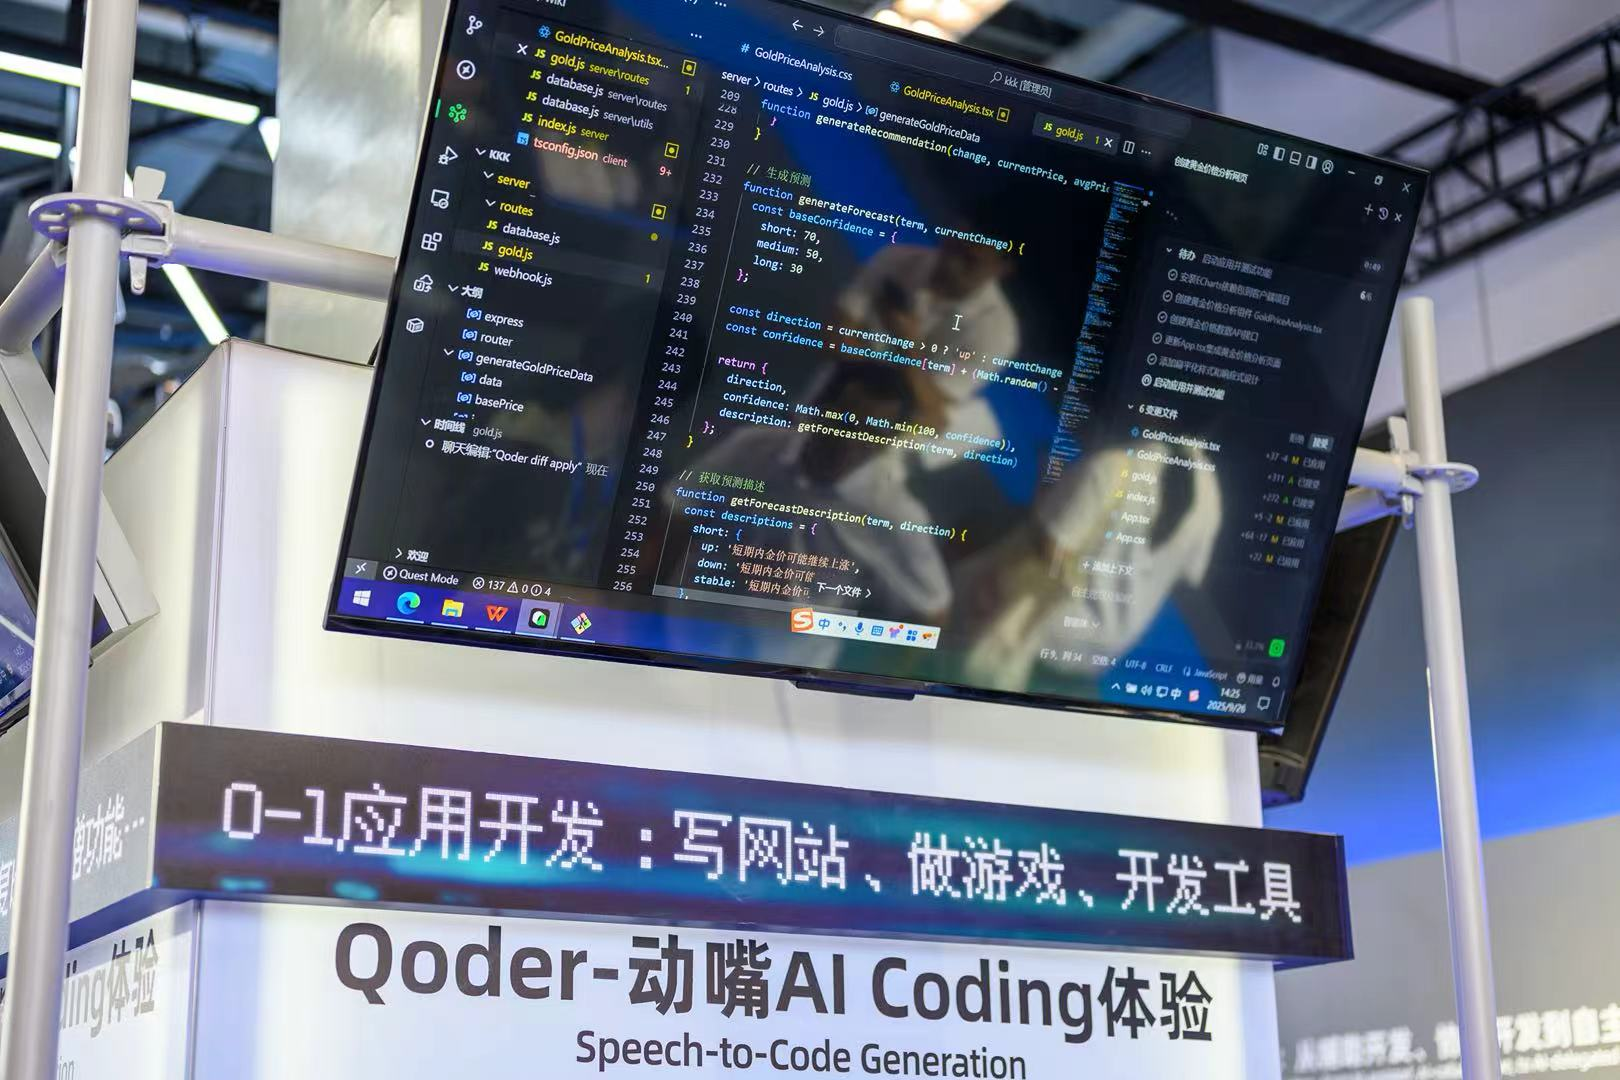
\includegraphics[width=.4\textwidth]{./fig/qoder.jpg}\quad
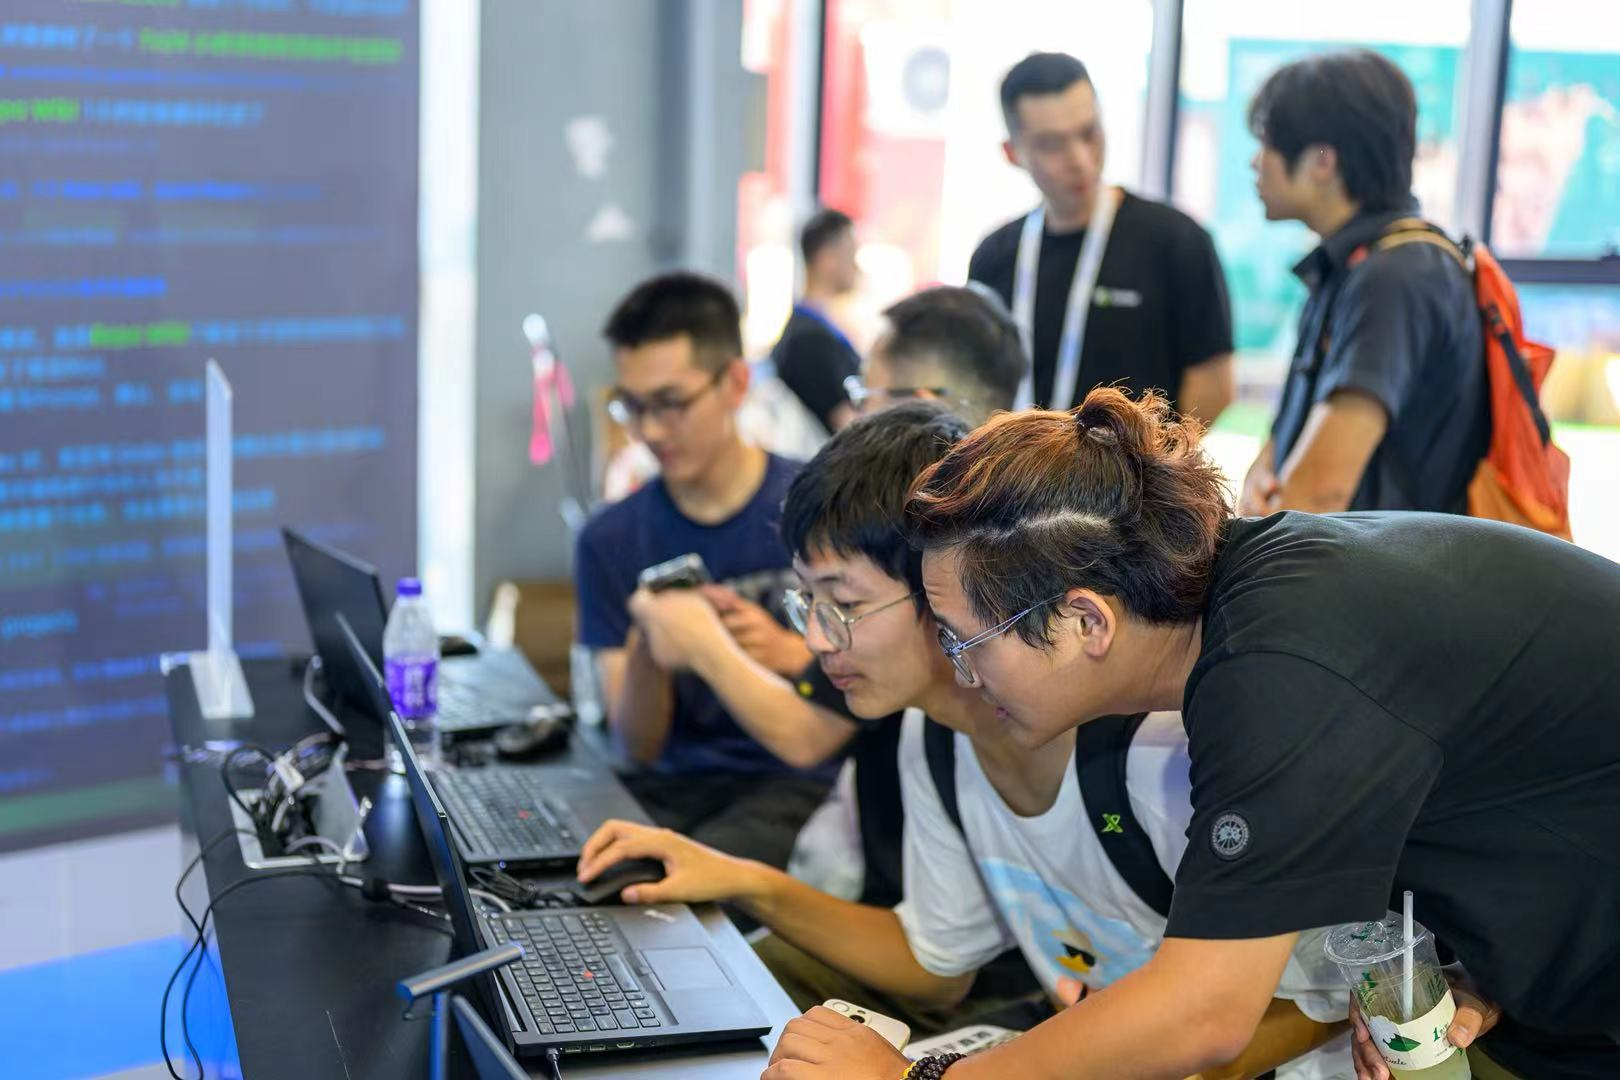
\includegraphics[width=.4\textwidth]{./fig/体验.jpg}
\caption{Qoder，同学们在积极体验，最后成功写了一个个人信息展示网页}
\end{figure}


那是一幅开发者与AI进行思想对谈的图景：你只需用自然语言描述一个功能，甚至一种感觉，AI便能心领神会地实时生成代码，并以灵动的可视化方式呈现。
这预示着软件工程的未来，工程师的角色将发生一场深刻的进化。我们或许不再是代码的砌砖工，逐行堆砌逻辑的壁垒，而是升华为思想的建筑师，与AI这一不知疲倦的伙伴并肩，专注于更高维度的创意、设计与系统构建。
这并非冰冷的机器取代，而是一种温暖的人机共生，是将人类从重复的劳作中解放，去拥抱更广阔的创造星空。

然而，这场数字盛宴并未让我迷失于虚拟的浮光。
英特尔、AMD与英伟达的展台，如同一座座坚实的岛屿，时刻提醒着我：一切数字世界的澎湃浪潮，皆源于物理世界的坚实地基。
\begin{figure}[H]
\centering
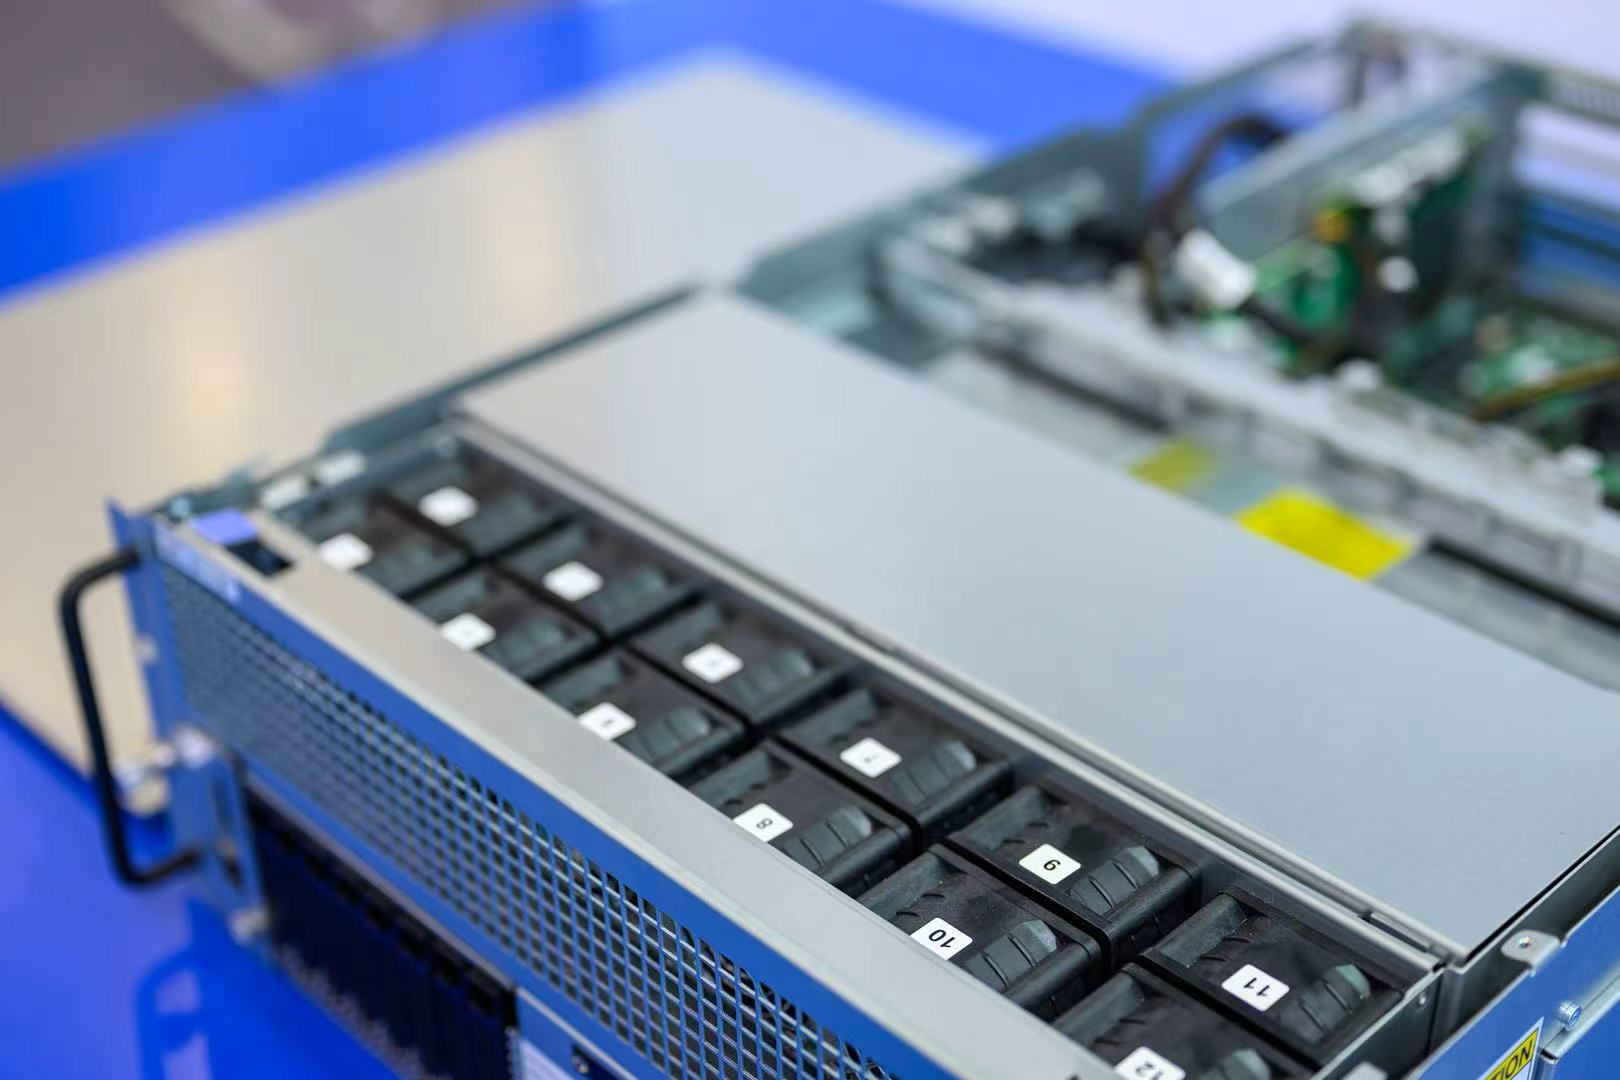
\includegraphics[width=.4\textwidth]{./fig/主机.jpg}\quad
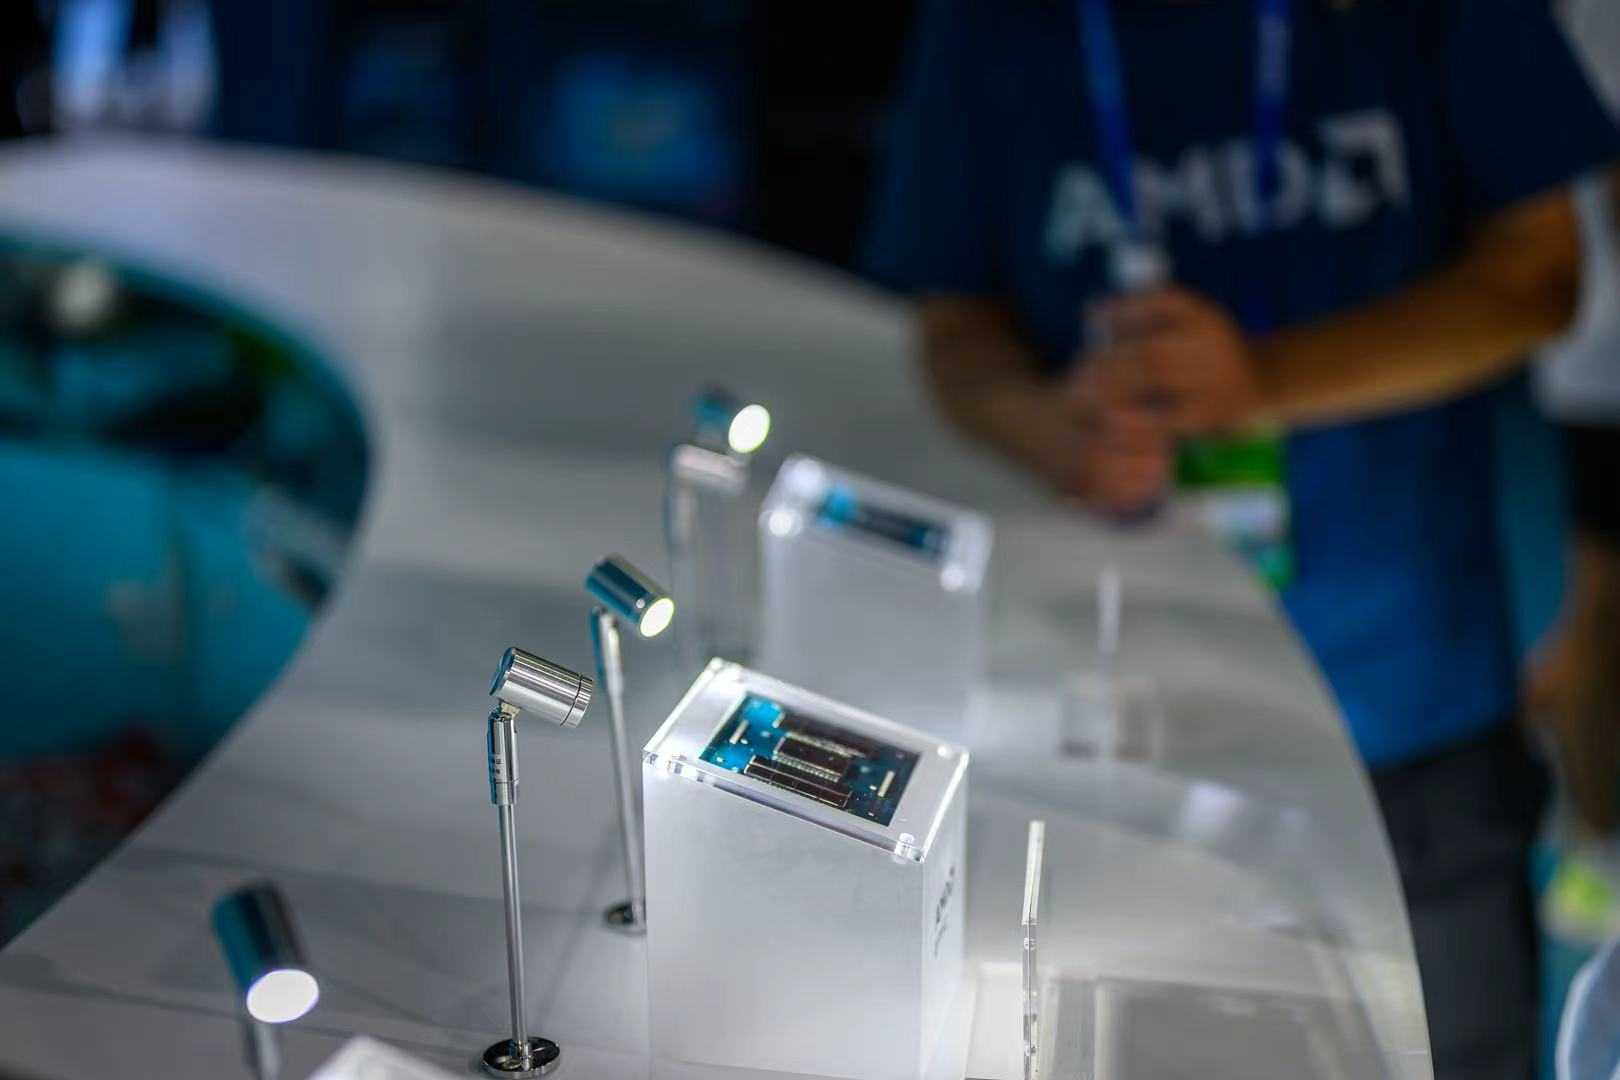
\includegraphics[width=.4\textwidth]{./fig/芯片.jpg}
\caption{参展的硬件厂商们纷纷拿出了他们针对AI的解决方案，是“AI”这个大工程的筑基者}
\end{figure}

那些在灯光下熠熠生辉的芯片，便是驱动人工智能思考的强大心脏。工程师们凭借鬼斧神工般的技艺，在方寸硅片之上，蚀刻出数百亿个晶体管的微观宇宙，赋予机器无与伦比的并行计算伟力。
从设计、流片到封测，这条精密至纳米的产业链，是半导体工程、材料科学与精密制造等顶尖学科的智慧结晶。正是这些由原子精密排列构成的硬件基石，为比特的自由奔腾和智能的绚烂涌现提供了可能。
在云栖大会这个数字为王的舞台上，我却前所未有地清晰洞见了虚拟与现实之间那份血脉相连的深刻羁绊。工程的广度与深度，正在这种从底层物理到顶层应用的层层递进与紧密耦合中，展现得淋漓尽致。

\begin{figure}[H]
\centering
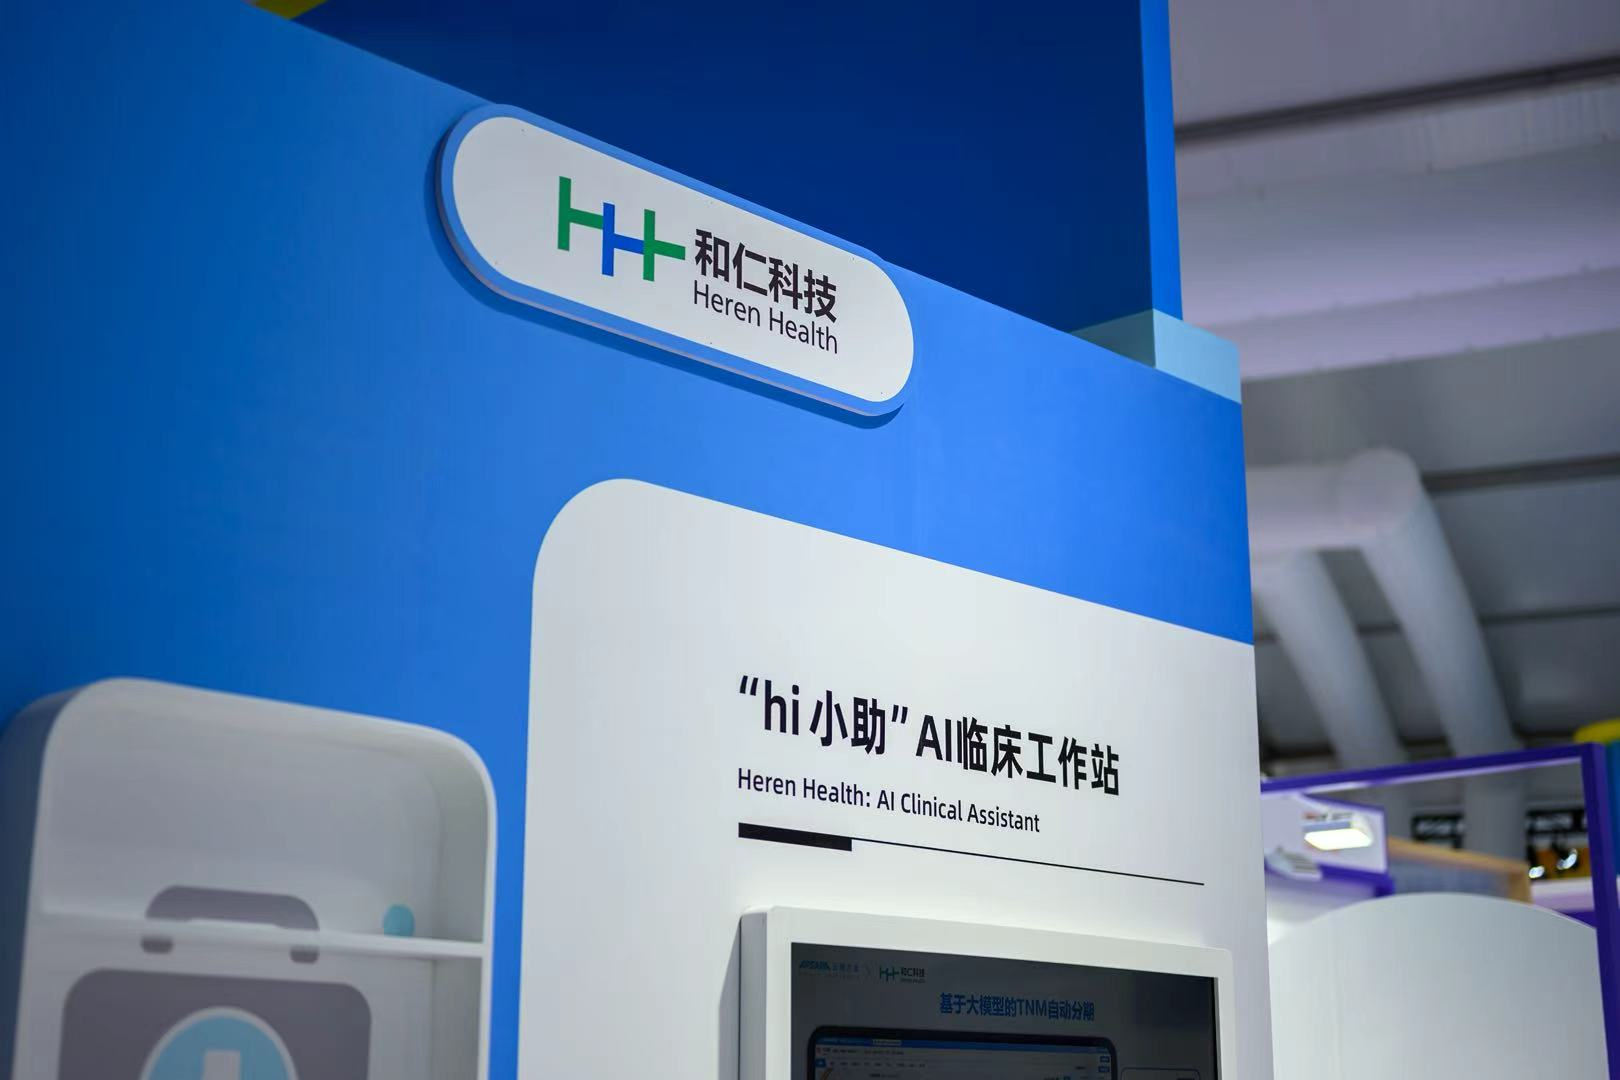
\includegraphics[width=.7\textwidth]{./fig/医疗.jpg}\quad
\caption{AI与医疗的结合，更是一项大工程}
\end{figure}


\section{工博会}
怀揣着这份对数实相依的全新感悟，我走进了上海工博会。
云栖的轻灵与无形，在此被工博会的厚重与坚实所取代。
巨大的展馆内，机器的低吼与机械臂的运转声交织成一曲雄浑的工业交响。
在这里，工程回归了它最经典、最宏大的叙事：驾驭物质与能量，塑造我们身处的物理世界。

工业自动化展区，是未来工厂的生动预演。
钢铁巨人般的工业机器人，以超越人类的效率和精度，精准地执行着焊接、搬运与装配的指令。
它们是现代制造业的中流砥柱，是智慧工厂的钢铁骨骼。其中，非夕科技的展台前，一幕场景令我叹为观止：一台柔性自适应机器人，以一种近乎艺术的优雅，用末端工具在脆弱的鸡蛋壳上进行精细雕刻。
这并非一次单纯的技术炫技，它象征着现代工业正从标准化、大批量的刚性生产，向着定制化、小批量的柔性制造深刻转型。
那金属手臂能够在触碰蛋壳的瞬间，感知细微的力反馈，并实时调整姿态与力度，这背后是传感器技术、控制算法与机器学习的无缝融合。
这已非简单的自动化，而是注入了感知、决策与适应能力的智能化自动化。
我看到，工程的未来不仅书写在云端的代码里，也镌刻在车间的钢铁之躯上，两者正以不同的姿态，共同驱动着生产力的伟大变革。
\begin{figure}[H]
\centering
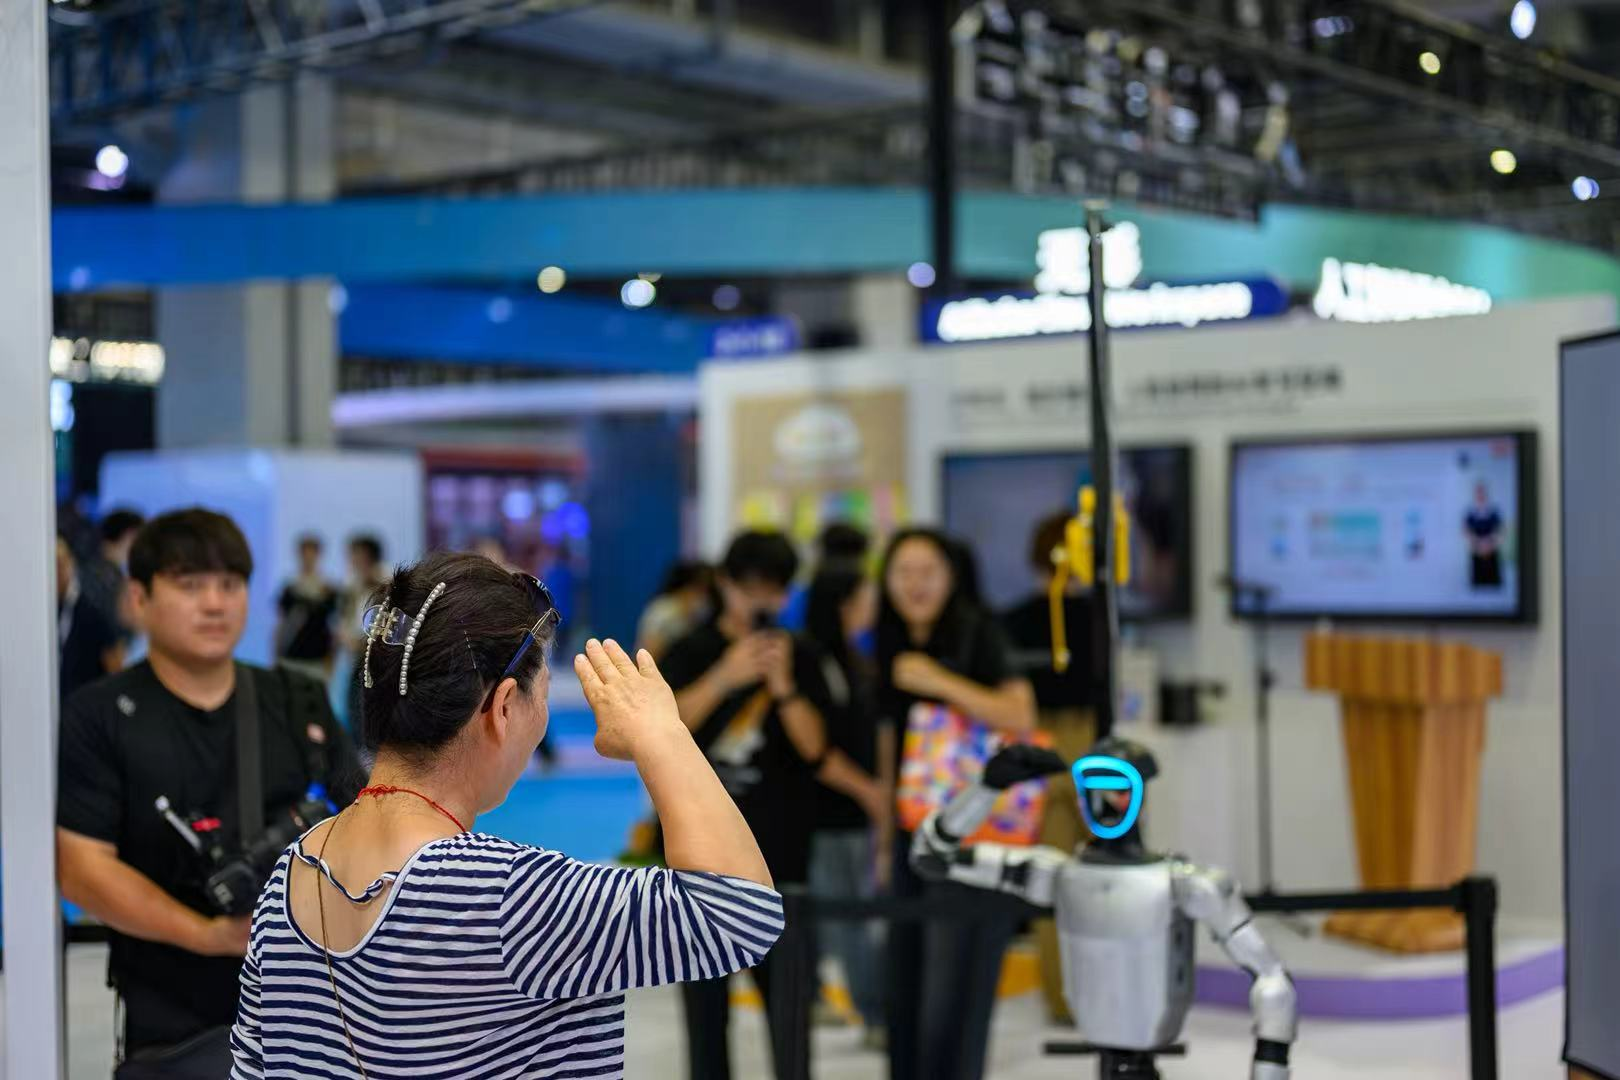
\includegraphics[width=.7\textwidth]{./fig/机器人.jpg}\quad
\caption{机器人精确模仿人的动作，展示其科技水平高超}
\end{figure}
移步至数控机床与金属加工展，我仿佛探入工业体系的更深腹地。
\begin{figure}[H]
\centering
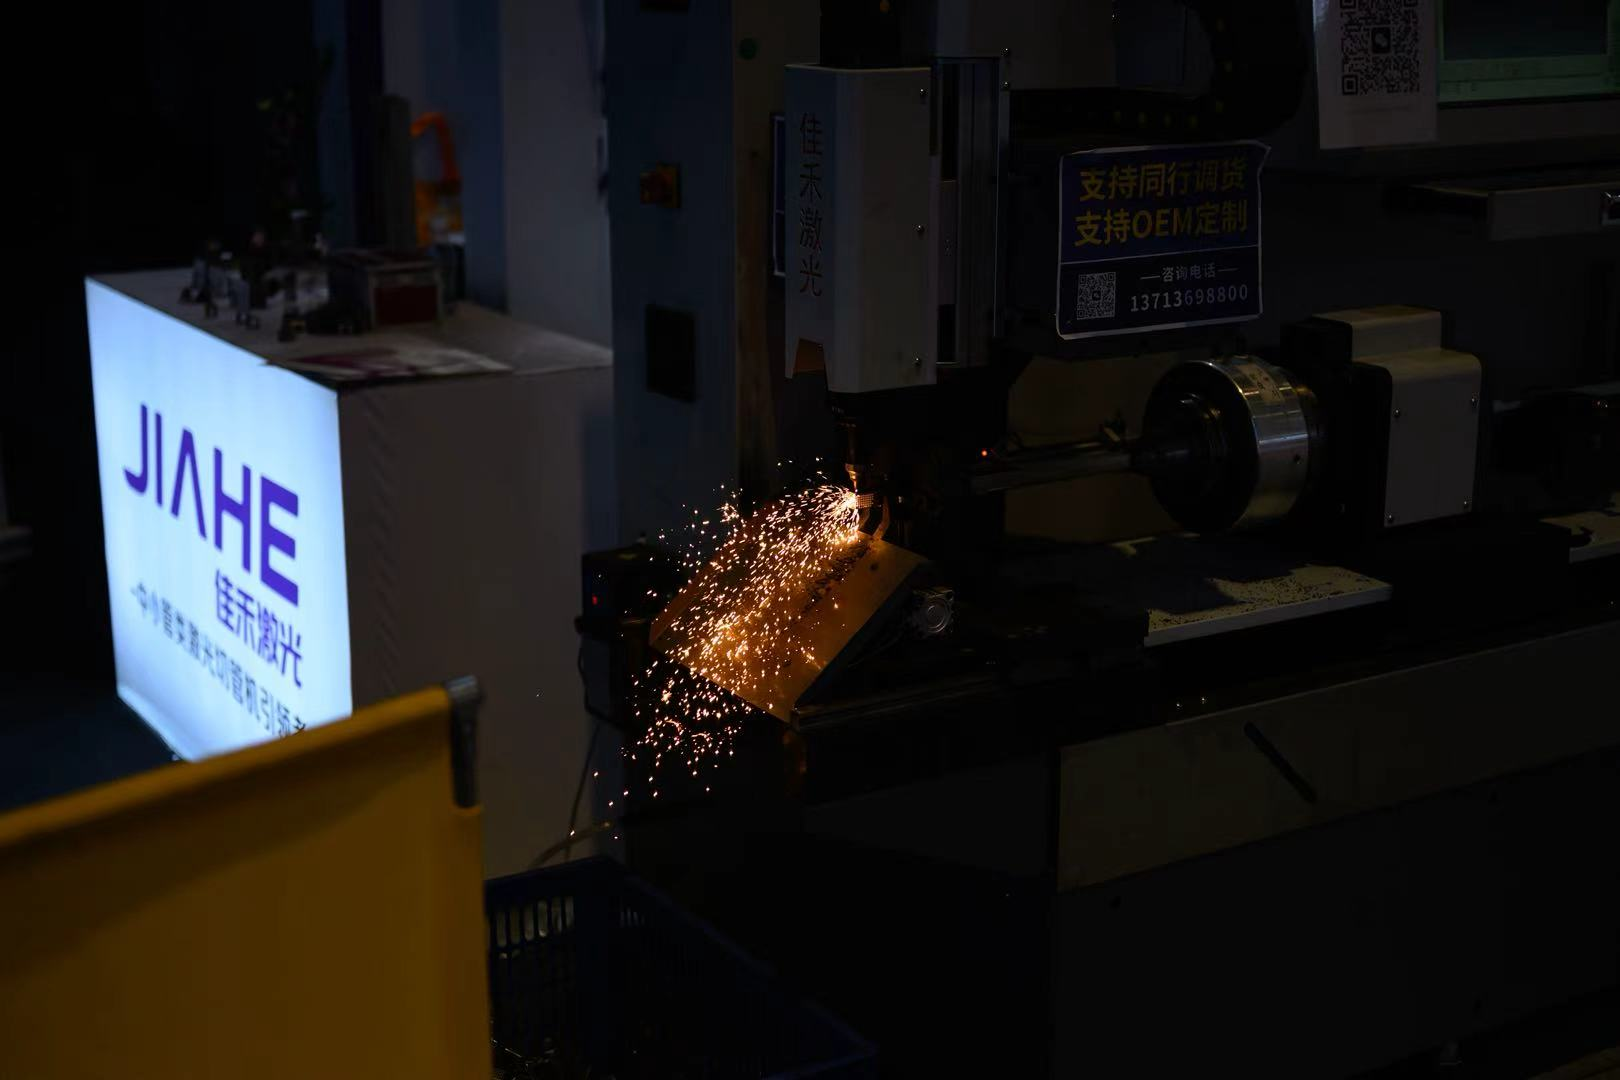
\includegraphics[width=.7\textwidth]{./fig/切削.jpg}\quad
\caption{激光切削}
\end{figure}

如果说机器人是制造业的肌肉与双手，那么这里的数控机床与激光切割设备，便是锻造这些肌体的“工业母机”。
它们是国家制造能力的基石，是整个工业金字塔最坚实的底座。目睹一台巨大的激光切割机在厚重钢板上游走，如热刀切开黄油般流畅，留下的切口光洁如镜，我深刻体会到工程的层级之美。
一个国家工业的崛起，离不开这些底层核心装备的自立自强。这些看似传统的机械工程领域，实则每天都在发生着革新。
更高精度的传感、更稳定的控制、更耐用的材料，每一个细微的进步，都将沿着产业链层层放大，最终支撑起整个高端制造业的宏伟大厦。
我对工程的敬畏，也因此多了一份对深厚根基的理解。它不仅包含前沿的璀璨，更包含那些深藏于产业根脉、沉默却不可或缺的基础力量。

旅程的终点，是科技创新展。
这里像一幅徐徐展开的画卷，将工程对现代社会的全面渗透与深刻塑造展现得淋漓尽致。
从守护家庭温馨的智能家居，到叩问深空的航空航天；从延续生命希望的尖端医疗设备，到重塑城市脉搏的新能源汽车。
\begin{figure}[H]
\centering
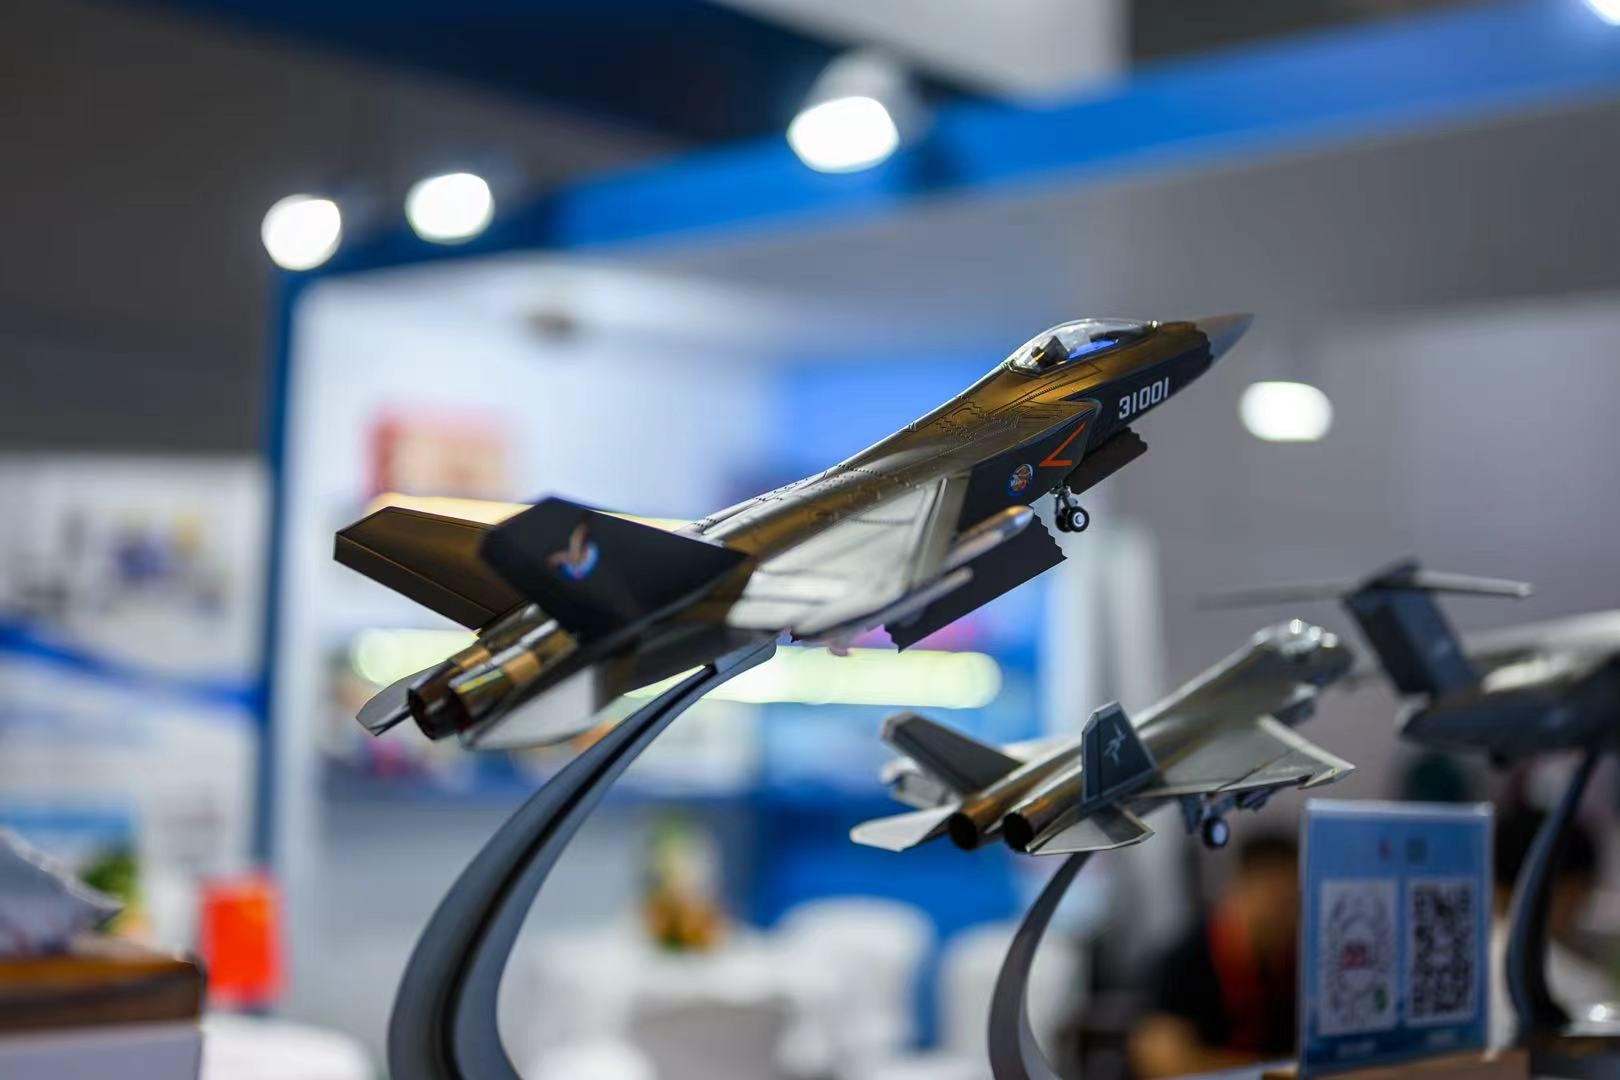
\includegraphics[width=.3\textwidth]{./fig/飞机.jpg}\quad
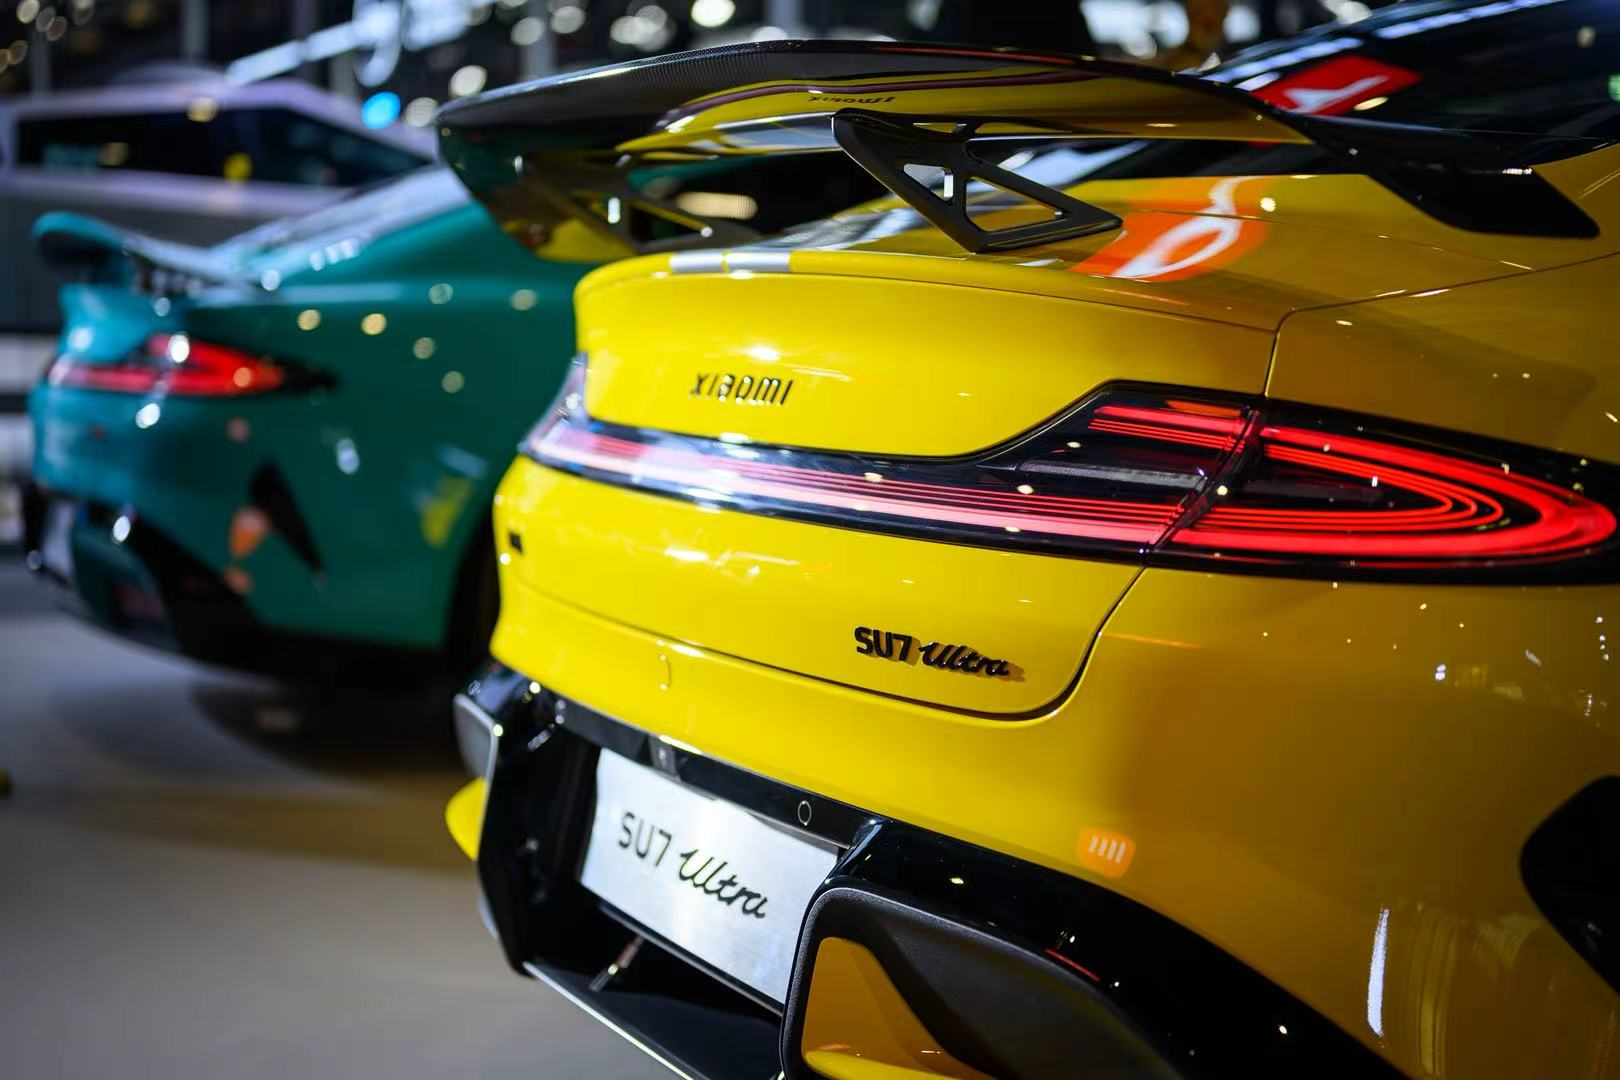
\includegraphics[width=.3\textwidth]{./fig/车.jpg}\quad
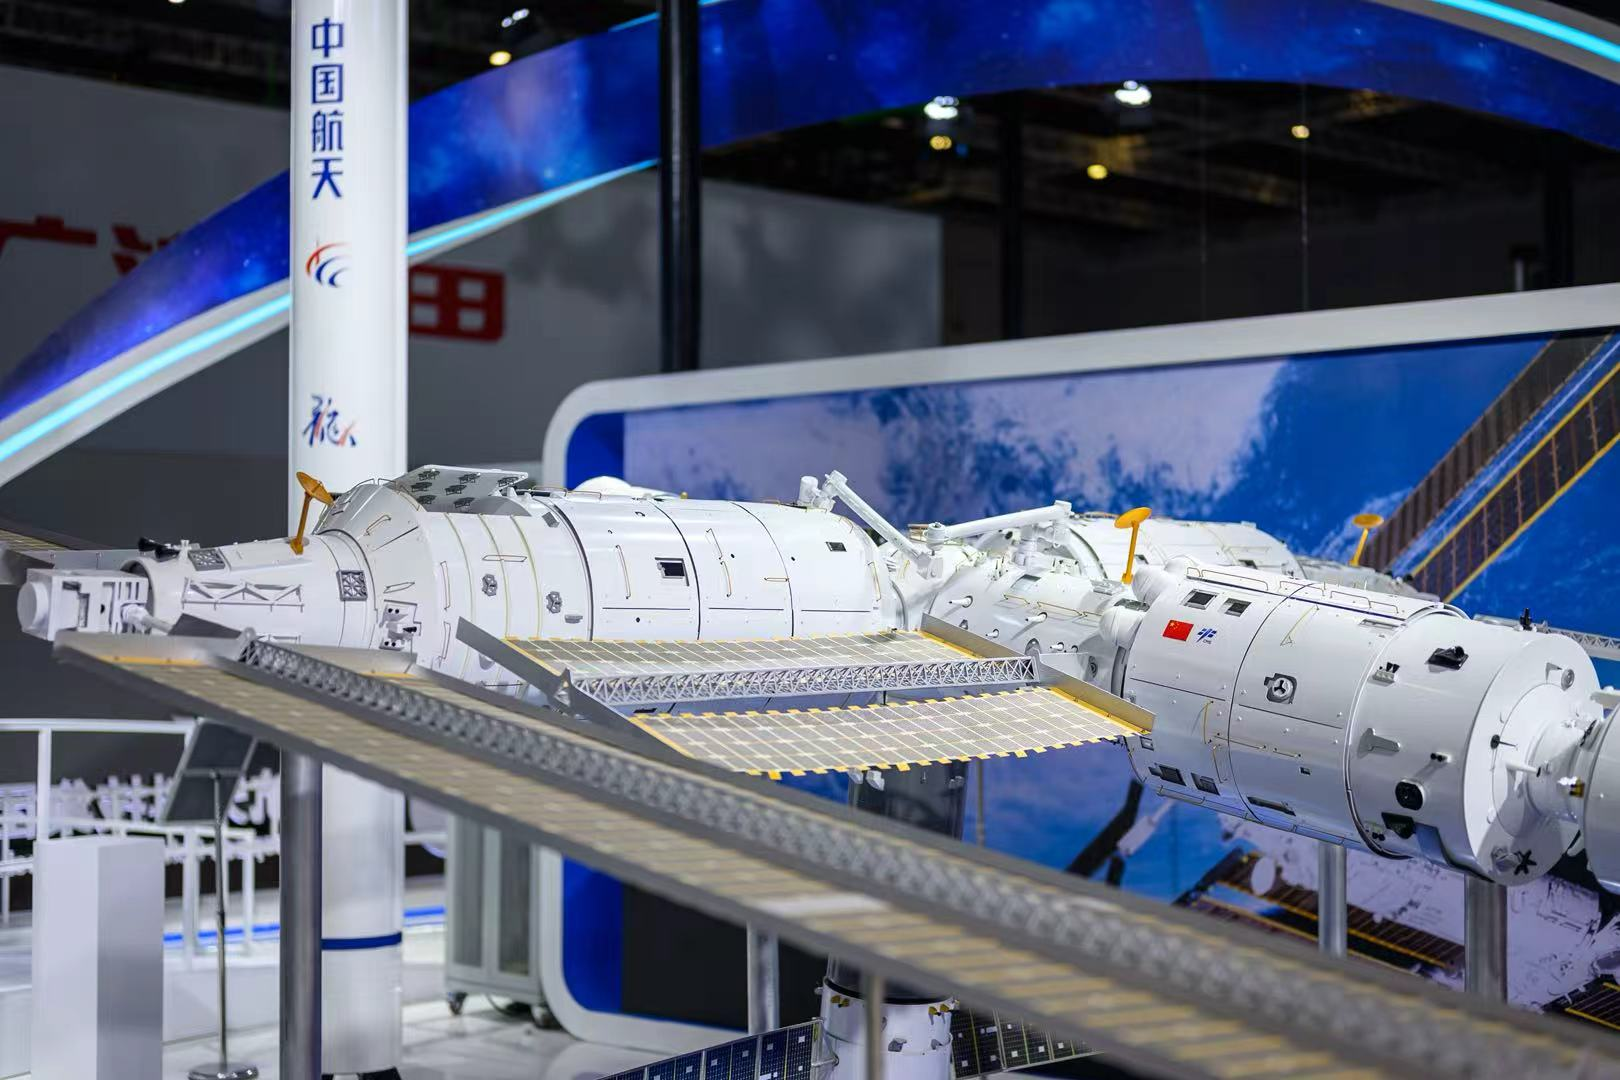
\includegraphics[width=.3\textwidth]{./fig/火箭.jpg}\quad
\caption{工业，工程所涵盖的内涵之广}
\end{figure}

每一项重大创新成果，都是一个庞大工程体系的缩影。一架翱翔天际的飞机，是空气动力学、材料科学、控制工程等无数智慧的结晶；一个聪慧体贴的智能家居系统，则是物联网、云计算与人工智能的完美交融。
在这里，工程的范畴被延展至无穷，它无处不在，它就是构建我们现代文明的筋骨与血脉。

\section{总结}
从云栖到工博，这场在比特与原子之间的穿行，最终在我心中融合成一幅完整而流动的工程新图景。
我意识到，工程的范畴，再也不是学科名录上那些孤立的条目。它是一个从最底层的物理法则，到中间层的实体工具，再到最上层的数字智能与服务的连续统一体。
数字世界与物理世界不再是遥遥相望的两个平行时空，它们正通过工程这座宏伟的桥梁，实现前所未有的深度融合。云端的算法指导着工厂的节拍，车间的数据滋养着模型的智慧。
这种数实共生的新形态，正是当代工程最核心的特征与最广阔的舞台。

而工程的未来，它的航向已无比清晰地指向了“智能”与“协同”的灯塔。
无论是云栖大会上席卷一切的人工智能，还是工博会上日渐聪慧的工业机器人，都昭示着智能化是所有工程领域不可逆转的洪流。
未来的工程造物，将不再是冰冷的工具，而是能够感知、认知、决策的智能伙伴。未来的工程过程，将是人与机器、机器与机器之间更深层次的和谐共舞。
工程师与AI共同谱写代码的乐章，设计师与机器人协同完成创造的雕塑。这必将极大地解放人类的创造潜能，赋予我们挑战更宏大、更复杂工程难题的勇气与能力。

这次参观，彻底重塑了我对工程的认知。
它并非一门静止的学科，而是一个生生不息、持续进化、不断拓宽自身边界的生命体。
它既能上九天揽月，亦可于蛋壳雕花；它既根植于坚实的物理大地，又在虚拟的数字苍穹中绽放无限光华。
作为一名即将投身于这个伟大领域的学子，我的内心充满了前所未有的激动与沉甸甸的责任。
我们正处在一个比特拥抱原子、智慧融入万物的时代。
未来的工程师，注定要成为这两个世界的沟通者、构建者与梦想家。我们的使命，已不再是仅仅遵循既有的定律与公式，而是在这片无垠的疆域里，以智慧为帆，以实干为桨，去创造、去担当，去构建一个更加智能、更加美好的未来世界。
这，或许正是《工程导论》这门课程，引领我们穿越理论的迷雾，想要亲手触摸到的、最真实、最滚烫的答案。
\end{document}
